\newpage
\clearpage
\section{Segmentação de Instâncias}
\label{instance:instance}

Sendo criada a partir de conceitos de segmentação semântica \cite{Minaee2021}, assim como atividades relacionadas à detecção de objetos, o qual é exemplificado pelo trabalho de \cite{Vaillant1994}, as segmentações de instâncias foram criadas com o intuito de segmentar objetos de uma imagem e separá-los quando representarem objetos de mesma classe, mas diferentes \cite{Hafiz2020}, algo que se torna de fácil entendimento ao visualizar a Figura \ref{instance:fig:4}.

\begin{figure}[H]
   \caption{Exemplos de segmentação de instâncias.}
   \centering
   \label{instance:fig:4}
    \begin{subfigure}[t]{0.45\textwidth}
        \centering
        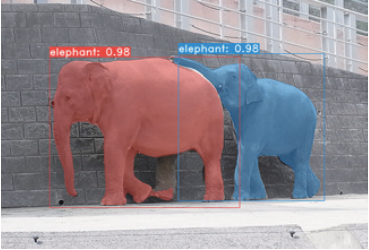
\includegraphics[height=1.3in]{recursos/imagens/instance/ins1.png}
        \label{instance:fig:4.1}
    \end{subfigure}%
    ~ 
    \begin{subfigure}[t]{0.45\textwidth}
        \centering
        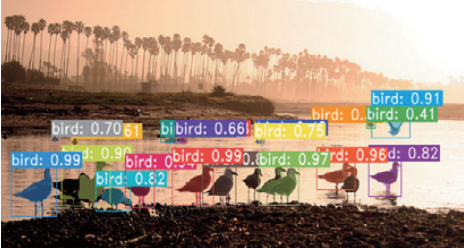
\includegraphics[height=1.3in]{recursos/imagens/instance/ins3.png}
        \label{instance:fig:4.2}
    \end{subfigure}%
    ~ 
    
    \begin{subfigure}[t]{0.45\textwidth}
        \centering
        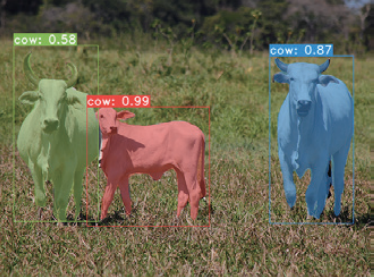
\includegraphics[height=1.3in]{recursos/imagens/instance/ins2.png}
        \label{instance:fig:4.3}
    \end{subfigure}
    ~
    \begin{subfigure}[t]{0.45\textwidth}
        \centering
        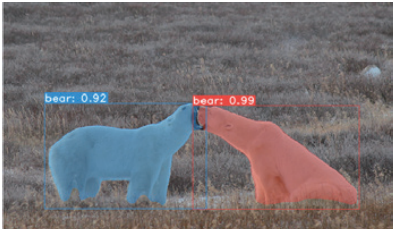
\includegraphics[height=1.3in]{recursos/imagens/instance/ins4.png}
        \label{instance:fig:4.4}
    \end{subfigure}

    \vspace*{1 cm}
    Fonte: retirado e adaptado de \cite{Bolya2019}.
\end{figure}

É relevante dizer que as atividades de segmentação de instâncias habitualmente ocorrem a nível de pixel e com uso de técnicas de CNN, que proporcionaram ainda mais competência para a evolução dessa categoria de segmentação.

Além disso, subcategorias de técnicas de segmentação de instâncias são comentadas por \cite{Hafiz2020}, das quais pode-se citar técnicas baseadas em máscaras, a técnica de detecção seguida por segmentação, classificação de pixels seguida de agrupamento e, finalmente, métodos de deslizamento denso de janelas, sendo que o primeiro citado é o mais explorado.

Sendo assim, neste Capítulo, estaremos tratando das métricas utilizadas para calcular o desempenho de modelos que utilizam de segmentação de instâncias (Seção \ref{instance:metrics}), bem como o modelo que representa o estado da arte para esse tipo de atividade (Seção \ref{instance:mask}).


\subsection{Métricas}
\label{instance:metrics}

No tocante às métricas que são utilizadas para a avaliação dos modelos de segmentação de instâncias, vale dizer que comumente são utilizadas as métricas de avaliação descritas pelo COCO \cite{Lin2016}, as quais habitualmente são utilizadas para o contexto de detecção de objetos e também englobam técnicas que já foram descritas para segmentação semântica (como descrito na Seção \ref{semantic:metrics}).

Todavia, dentre as métricas mais utilizadas para essa categoria de segmentação, cita-se a de \textit{average precision} que será detalhada a seguir (Seção \ref{instance:AP}).


\subsubsection{\textit{Average Precision}(AP)}
\label{instance:AP}

A métrica de precisão média, do inglês, \textit{average precision} (AP) é amplamente utilizada para os conceitos de detecção de objetos, sendo utilizada até mesmo para redes \textit{Fast} R-CNN \cite{Girshick2014} e SSD \cite{Liu2015a}. Para que o cálculo da AP seja realizado, conceitos de precisão (Equação \ref{semantic:eq:3}) e revocação (Equação \ref{semantic:eq:4}) são necessários, visto que AP é definida como a área abaixo da curva de precisão e revocação \cite{Hariharan2014} que está exemplificada na Figura \ref{instance:fig:1}.

\begin{figure}[H]
    \centering
    \caption{Representação de curvas de precisão e revocação.}
    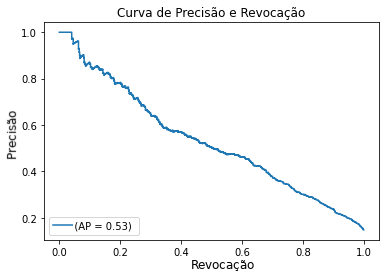
\includegraphics[height=2.3in]{recursos/imagens/instance/precisao_revocacao.png}
    \label{instance:fig:1}

    \vspace*{1 cm}
    Fonte: do próprio autor.
\end{figure}

Dessa forma, AP pode ser definida pela Equação \ref{instance:eq:1}:

\begin{equation}
    \label{instance:eq:1}
    \text{AP} = \sum_n (R_n - R_{n-1}) P_n,
\end{equation}
sendo que o valor de $AP$ estará em um domínio $[0,1]$, além de ter $P_r$ e $R_n$ representando precisão e revocação, respectivamente.

Por fim, vale dizer que variações também são utilizadas para a métrica de AP, por exemplo, a métrica \textit{Mean Average Precision} (mAP), sendo que essa calcula a média de todas as APs de todas as classes encontradas em determinada imagem.


\subsection{\textit{Mask} R-CNN}
\label{instance:mask}

Criada como uma extensão do modelo \textit{Faster} R-CNN \cite{Ren2017} (como é possível observar na Figura \ref{instance:fig:5}), o \textit{framework} considerado estado-da-arte para tópicos relacionados à segmentação de instâncias foi nomeado de \textit{Mask} R-CNN \cite{He2020}, o qual conseguiu resultados relevantes nos desafios COCO \cite{Lin2016}, sendo que diferente de atividades relacionadas à detecção de objetos, que oferecem apenas uma caixa delimitadora (\textit{bounding box}) e a classificação do objeto em questão, quando se trata do \textit{framework} \textit{Mask} R-CNN, há um mascaramento em relação aos formatos dos objetos detectados, assim como a possibilidade de diferenciação entre as instâncias \cite{Hafiz2020}.

\begin{figure}[H]
    \centering
    \caption{Evolução de modelos até o \textit{Mask} R-CNN.}
    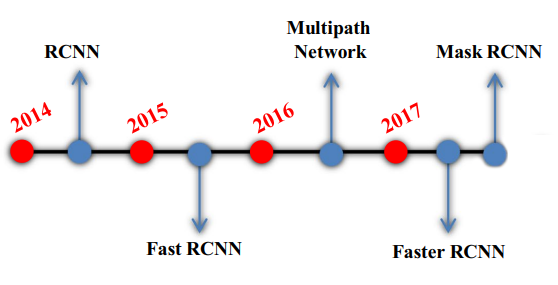
\includegraphics[height=2.3in]{recursos/imagens/instance/mask_rcnn_evol.png}
    \label{instance:fig:5}

    \vspace*{1 cm}
    Fonte: retirado e adaptado de \cite{Hafiz2020}.
\end{figure}

Quanto a esse \textit{framework}, vale ressaltar que o mesmo possui três ramos principais em sua arquitetura \cite{He2020, Minaee2021}, que são representados na Figura \ref{instance:fig:2}, sendo que dois deles também estão presentes em modelos que utilizam do \textit{Faster} R-CNN \cite{Ren2017}. O ramo principal que é executado pelo modelo \textit{Mask} R-CNN é o de predição de máscara em relação ao objeto de interesse e as outras duas são as classes dos objetos e as coordenadas das \textit{bouding boxes} \cite{Minaee2021}.

\begin{figure}[H]
    \centering
    \caption{Representação do \textit{Mask} R-CNN para segmentação de instancias.}
    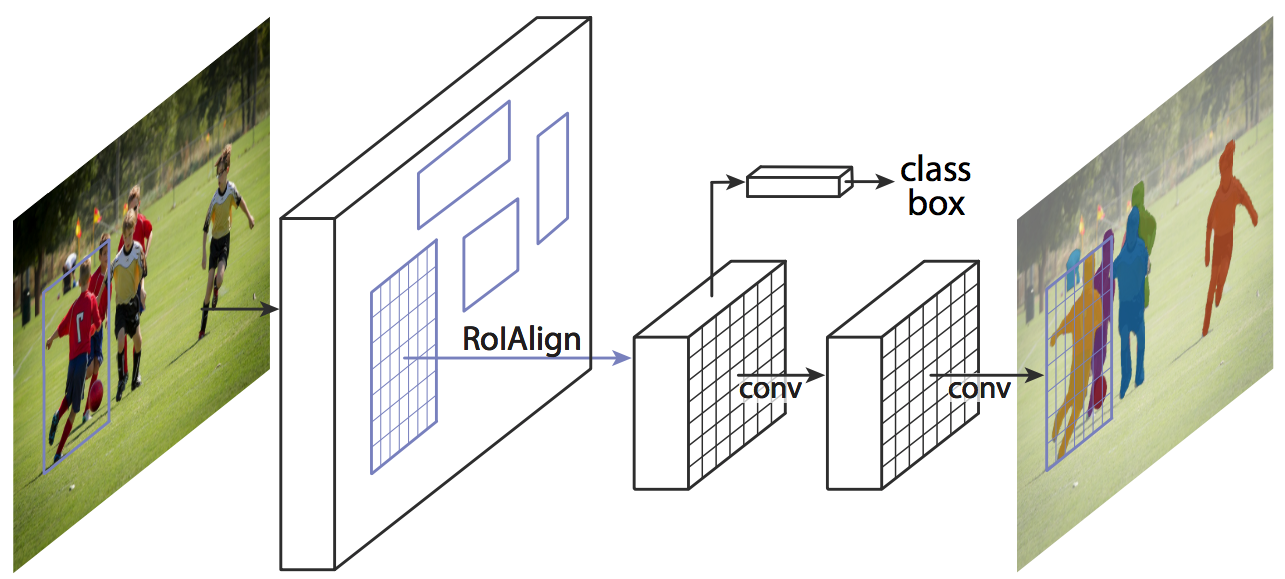
\includegraphics[height=2.3in]{recursos/imagens/instance/Mask-R-CNN_examp.png}
    \label{instance:fig:2}

    \vspace*{1 cm}
    Fonte: \cite{He2020}.
\end{figure}

Por fim, destaca-se nesses modelos o seu desempenho, visto que com a arquitetura proposta por \cite{He2020}, é possível executar o modelo em cenas à 5 \textit{frames} por segundo - GPU não especificada pelo autor - \cite{Minaee2021, He2020, Hafiz2020}, além do fato que o modelo explora as técnicas de CNN (Seção \ref{deep:CNN}) para sua otimização \cite{Li2020}, possibilitando o seu uso até mesmo em outras tarefas fora do contexto de segmentação, como as atividades de estimação de pose. As imagens que representam o uso do \textit{framework} \textit{Mask} R-CNN podem ser observadas na Figura \ref{instance:fig:3}.

\begin{figure}[H]
    \centering
    \caption{Exemplos de uso do \textit{Mask} R-CNN.}
    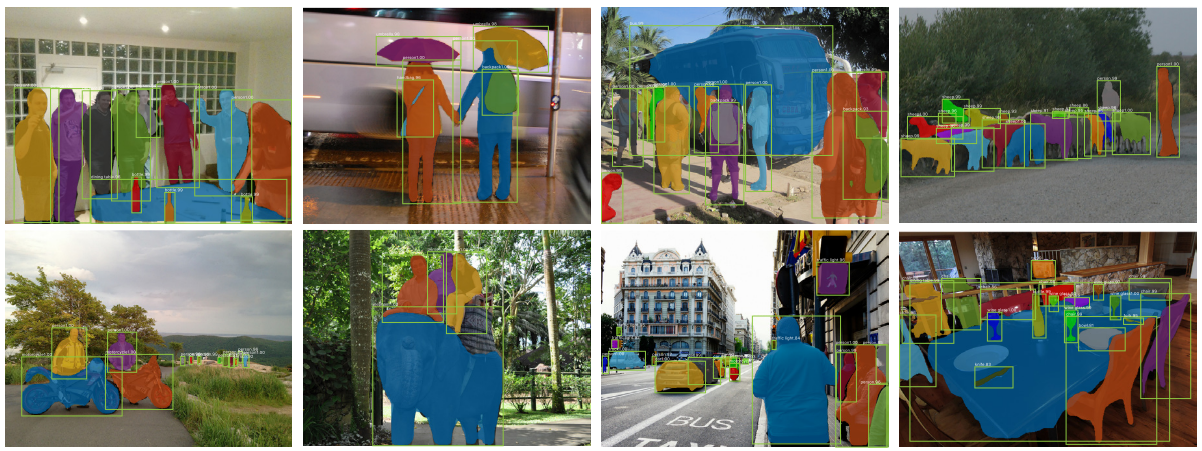
\includegraphics[width=1\textwidth]{recursos/imagens/instance/insta_examp.png}
    \label{instance:fig:3}

    \vspace*{1 cm}
    Fonte: \cite{He2020}.
\end{figure}


\subsection{Considerações Finais do Capítulo}
\label{instance:conclusion}

Por meio dos estudos realizados em relação à segmentação de instâncias, pôde-se perceber que há uma recomendação para fatores relacionados a alto desempenho, localização de objetos e mascaramento exato das regiões de interesse, não obstante, como dito por \cite{Kirillov2019a}, as segmentações de instâncias possuem uma deficiência quando há uma necessidade de segmentar cenas que não possuem um objeto em especifico como foco, por exemplo, paisagens em que tudo é denominado com o tipo de classificação \textit{stuff} (o que será detalhado no Capítulo \ref{panoptic:panoptic}).